\documentclass[11pt]{article}

%	packages
\usepackage{tikz}
\usepackage{authblk}
\usepackage{amsmath}
\usepackage{amssymb} 
\usepackage{caption}
\usepackage{graphicx}
\usepackage[hypertexnames=false,colorlinks=true,linkcolor=blue,citecolor=blue]{hyperref}
\usepackage[numbers,comma,square,sort&compress]{natbib}
\usepackage[a4paper,text={6.5in,10in},centering]{geometry}
\usepackage{subcaption}
%	code syntax higlighting
\usepackage{listings}
\usepackage{color}
\usepackage{textcomp}
\definecolor{listinggray}{gray}{0.9}
\definecolor{lbcolor}{rgb}{0.9,0.9,0.9}
% C++ = [Visual]C++ ; matlab = matlab
\lstset{
	backgroundcolor=\color{lbcolor},
	tabsize=4,
	rulecolor=,
	language=java,
	keywordstyle=\bfseries\ttfamily\color[rgb]{0,0,1},
	identifierstyle=\ttfamily,
	commentstyle=\color[rgb]{0.133,0.545,0.133},
	stringstyle=\ttfamily\color[rgb]{0.627,0.126,0.941},
	showstringspaces=false,
	basicstyle=\small,
	%numberstyle=\footnotesize,
	%numbers=left,
	stepnumber=1,
	numbersep=10pt,
	tabsize=2,
	breaklines=true,
	prebreak = \raisebox{0ex}[0ex][0ex]{\ensuremath{\hookleftarrow}},
	breakatwhitespace=false,
	aboveskip={1.5\baselineskip},
  columns=fixed,
  upquote=true,
  extendedchars=true,
 frame=single,
% backgroundcolor=\color{lbcolor},
}


%	figures
\graphicspath{{eps/}{pdf/}{../figs//}}
%\setcaptionmargin{0.25in}
\def\captionfont{\itshape\small}
\def\captionlabelfont{\upshape\small}

%	counters
\makeatletter\@addtoreset{equation}{section}\makeatother
\renewcommand{\theequation}{\arabic{section}.\arabic{equation}}


%%%%%%%%%%%%%%%%%%%%%%%%%%%%%%%%%%%%%%%%%%%%%%%%%%%%%%%%%%%%%%%%%%%%%%%%%%%%

\begin{document}

\title{Equation-free analysis of agent-based models:\\1-D Ising Model}

%\author[1]{Spencer A. Thomas}
\author{Spencer A. Thomas}
\author{David J.B. Lloyd}
\author{Anne C. Skeldon}
%\affil[1]{\small Department of Mathematics, Evolution and Resilience of Industrial Ecosystems (ERIE), University of Surrey, Guildford, GU2 7XH, UK}
\affil{\small Department of Mathematics, Evolution and Resilience of Industrial Ecosystems (ERIE), University of Surrey, Guildford, GU2 7XH, UK}
\date{\today}
\maketitle


%%%%%%%%%%%%%%%%%%%%%%%%%%%%%%%%%%%%%%%%%%%%%
% stochastic double well
%%%%%%%%%%%%%%%%%%%%%%%%%%%%%%%%%%%%%%%%%%%%%

\section{The Model: An Overview}
This is a model of a magnet based on the magnetic moments (spins) of the atoms it contains \cite{Ising} and is available in the NetLogo model library \cite{Netlogo}. In this model each element of a 2D lattice represents an atom (agent) in the magnet with a spin either up ($+1$) or down ($-1$). Each spin state can be influenced by the temperature of the magnet and the magnetic moment of four neighbouring atoms. The overall spin of the magnet, known as the magnetization ($M$), is based on the sum of the spins of $k$ atoms in the magnet,
	\begin{equation}
	M = \sum_{i=1}^k \delta_i, \quad ; \quad
 	\delta_i = \left\{
  \begin{array}{cl}
     1 &: \textit{spin up}\\
    -1 &: \textit{spin down}
  \end{array}
	\right. 
	. 
	\end{equation}


\begin{figure}[h]
        \centering
        		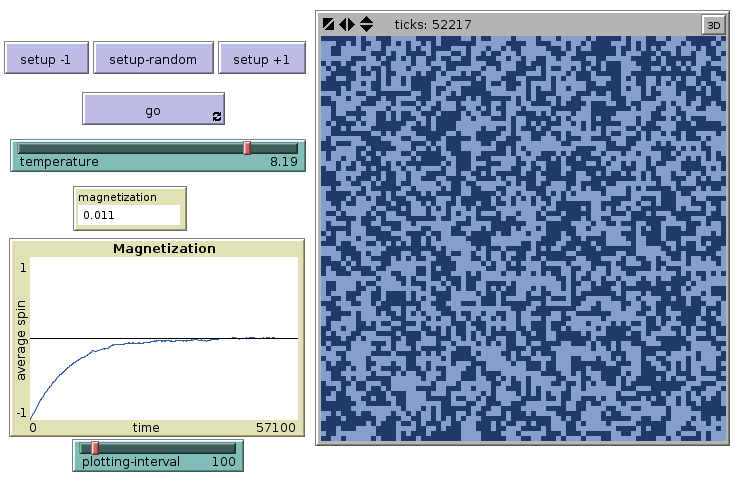
\includegraphics[width=\textwidth]{IsingInterface.png}
        \caption{1-D Ising model interface with one controllable parameter.\label{ising}}
\end{figure}



\section{The Model: Details} 
\label{sec:details}
The behaviour of the system is dependent on temperature $T$, in the low temperature limit the system is a ferromagnet and in the high temperature limit the system is in a paramagnetic state. The energy, $\epsilon$, of the atom at the $i,j$ location is defined as the negative sum of the product of the spin of an atom and its four neighbours ($nbh$);
 	\begin{equation}
 		\label{eq:IsingEpsilon}
		\epsilon_{i,j} = -\sum\limits^{nbh} \delta_{i,j}\delta_{nbh}~ 
		= -\delta_{i,j}\left(\delta_{i,j-1} + \delta_{i,j+1} + \delta_{i-1,j} + \delta_{i+1,j}\right)~.
	\end{equation}
	The energy is a measure of similarity or difference of an atom's spin state to that of its neighbouring atoms with a maximum value of $4$, where an atom is the opposite to all of its neighbours, and a minimum of $-4$, where all five atoms have the same spin state. The probability, $p$, of an atom changing to the opposing spin state is determined through the Metropolis algorithm; 
  	\begin{equation}
  		\label{eq:ising}
		p = e^{-\Delta\epsilon / T}~,
	\end{equation}	 
 	where $\Delta\epsilon$ is the difference in energy caused by an atom changing its spin state. That is the difference in Equation~(\ref{eq:IsingEpsilon}) between $\delta_{i,j}$ and $(-\delta_{i,j})$. Equation~(\ref{eq:ising}) states that the $p$ decreases for increasing $\Delta\epsilon$, but that $p$ also increases with $T$. This example represents an abstract model that can simulate phase-transition behaviours in physical and social sciences \cite{Ising}. Here we perform equation-free analysis by continuing in $T$ and computing $f(M^\ast;T) = M^\ast(T)$, the results of the continuation are given in Fig.~\ref{fig:Ising}. 


\section{Requirements of the User}
The user defined settings in the input file are given below. 
\begin{lstlisting}
String NetlogoFile = "netlogo/Ising.nlogo"; 
String[] systemParameters = {"set temperature"};
double[] param = {2.5}; 
String[] Measure	= {"magnetization"}; 
String[] LiftOperator = {"set magnetization"}; 
double[] Initial	= {0.0}; 
boolean isSystemInitialised = false; 
\end{lstlisting}		
	Here the {\tt NetlogoFile} is a string of text with the location of the NetLogo file, here contained in the sub-folder {\it netlogo}. {\tt Lift} is the name of the parameters required to set up with system, which correspond to the values in {\tt param}. Note the parameter you wish to vary in order to analyse the system with this package goes first in this list. {\tt systemParameters} are the parameters are the parameters you wish to monitor during this analysis which take the initial value of {\tt Initial} as an estimate of the first fixed point of the system. Note there can be any number of {\tt systemParameters} in your system. {\tt Measure} is the output measure of the system, note this is not the same as {\tt systemParameters} in general. 


The default model is available in the NetLogo model library, however can only initialise the state of the lattice with all atoms; spin up ($M$=+1), spin down ($M$=-1), or randomly orientated ($M$=0). In order to enable the appropriate macroscopic state to be lifted to the microscopic simulations, i.e. based on the previous fixed point, a small modification is made to the {\tt setup} procedure in the model. This modification (shown below) enables the magnitization $M$ to be initialised at any value [-1:+1] by defining {\tt initialM}, which is lifted from the macroscopic state.
\newpage
\begin{lstlisting}
to setup
  clear-all 
  ask patches [ lift ]	;;  new procedure in place of +/-1 or 0
  set sum-of-spins sum [spin] of patches
  reset-ticks
end
\end{lstlisting}	
Here we also include a new procedure, {\tt Lift}, to appropriately initialise the model.
\begin{lstlisting}
to lift 
  let ptype random-float 2.0
  let random-number ptype - 1.0 
  ifelse initialM < random-number [ set spin -1 ] [ set spin 1 ]
  recolor
end
\end{lstlisting}



\section{Outcome of Equation-free Analysis}


As illustrated in Fig.~\ref{fig:bifurcation}, the systems is fixed in the $\pm 1$ spin state until the temperature is above a threshold $\widetilde{T}=1$. Above this threshold for $T$ we see a dependency of the magnetisation fixed point with temperature. This is the ferromagnetic state where the system exhibits spontaneous magnetisation and converges to either stable branch. Which of these two state the system converges to is dependent on initial conditions.

\begin{figure}[h]
        \centering
      \begin{subfigure}[b]{0.5\textwidth}
   %   \includegraphics[width=0.75\linewidth]{IsingCrop}
      			\begin{tikzpicture}
      			  	\node[anchor=south west,inner sep=0] at (0,0) {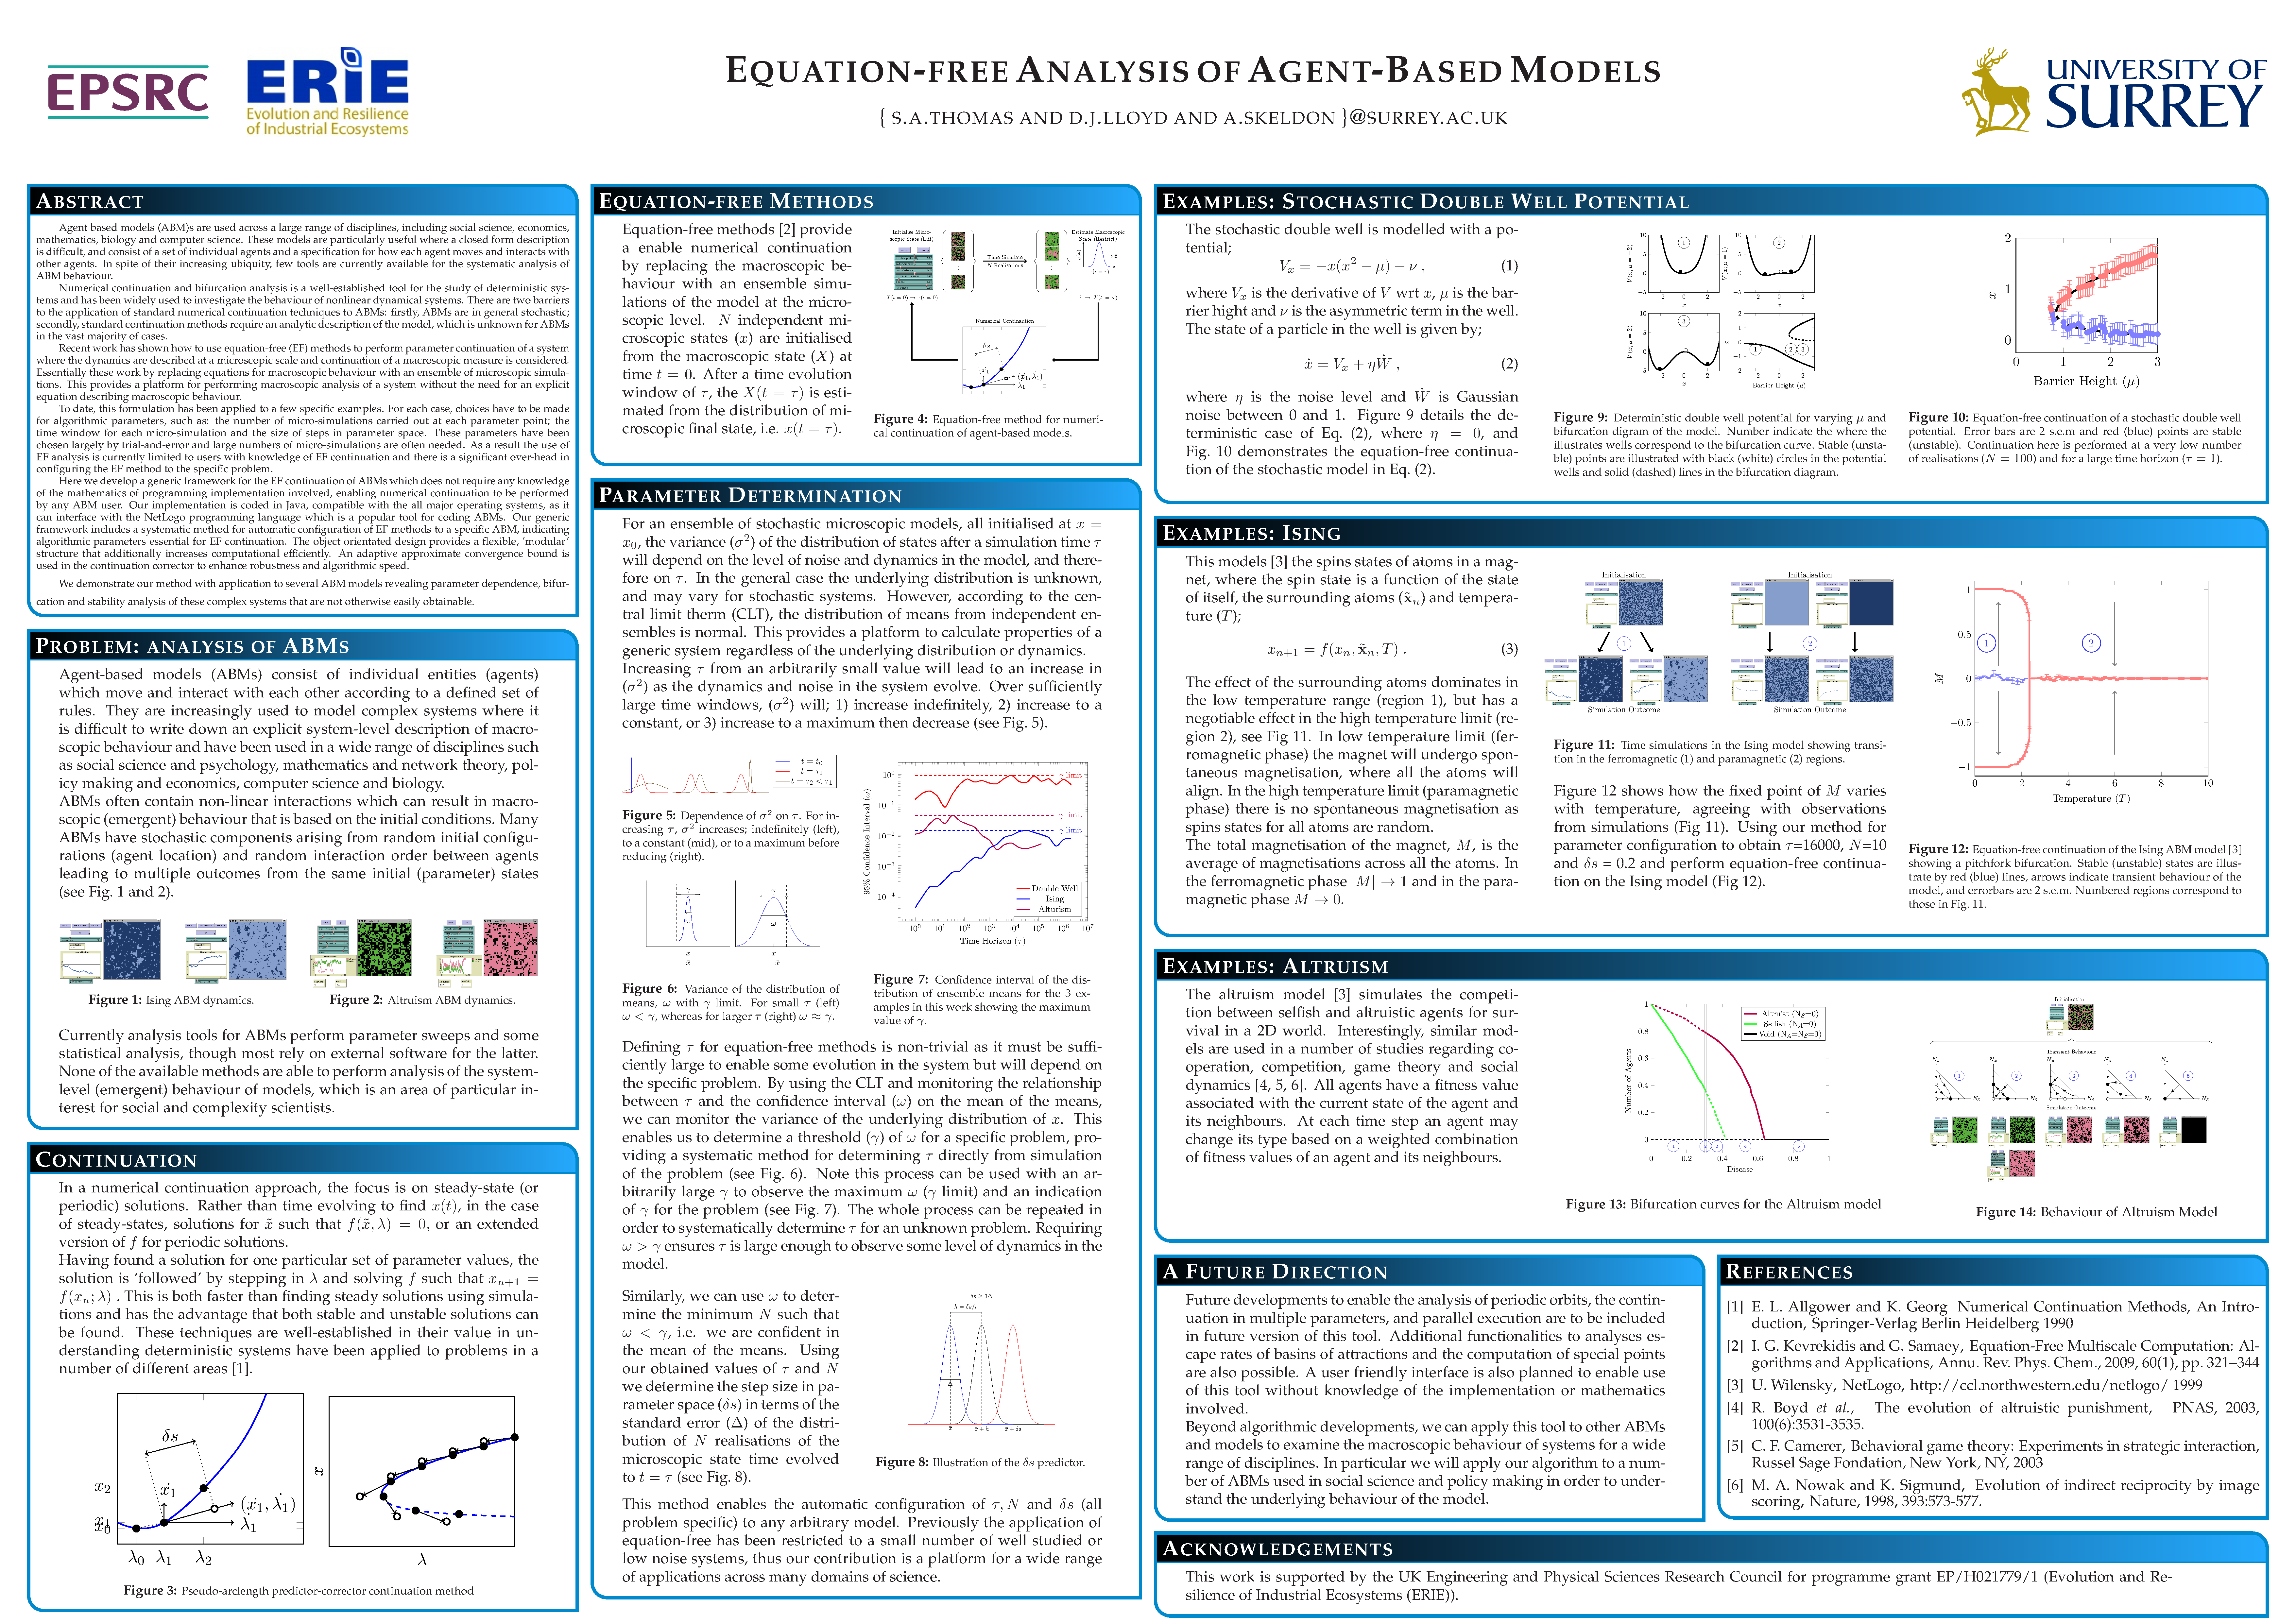
\includegraphics[width=\linewidth, trim=100cm 42cm 2cm 30cm, clip=true]{BMC2015.pdf}};
		    				
      				
              \node[] at (1.5,5.72) {\Large 1};
              \node[] at (1.5,3.5) {\Large 2};
              \node[] at (1.5,1.25) {\Large 3};
             
              \node[] at (2.5,5.22) {\Large 4};
              \node[] at (2.5,3.5) {\Large 5};
              \node[] at (2.5,1.75) {\Large 6};
              
              \node[] at (4.5,3.5) {\Large 7};
              \node[] at (5,3.5) {\Large 8};
              \node[] at (5.5,3.5) {\Large 9};
                \end{tikzpicture}
                \caption{Bifurcation}\label{fig:bifurcation}
     \end{subfigure}   
     \begin{subfigure}[b]{0.4\textwidth}  
        \begin{subfigure}[b]{0.3\textwidth}
        \begin{tikzpicture}
        	\node[anchor=south west,inner sep=0] at (0,0) {  
\includegraphics[width=\textwidth]{+1_T=0_tau=30k}};
        	\node[white] at (0.5,1.5) {\Huge 1};
        \end{tikzpicture}
     \end{subfigure}
     \begin{subfigure}[b]{0.3\textwidth}
        \begin{tikzpicture}
        	\node[anchor=south west,inner sep=0] at (0,0) {  
\includegraphics[width=\textwidth]{+1_T=2,27_tau=30k}};
        	\node[white] at (0.5,1.5) {\Huge 4};
        \end{tikzpicture}
     \end{subfigure}
     \begin{subfigure}[b]{0.3\textwidth}
        \begin{tikzpicture}
        	\node[anchor=south west,inner sep=0] at (0,0) {  
\includegraphics[width=\textwidth]{+1_T=7_tau=30k}};
        	\node[white] at (0.5,1.5) {\Huge 7};
        \end{tikzpicture}
     \end{subfigure}\\
     \begin{subfigure}[b]{0.3\textwidth}
        \begin{tikzpicture}
        	\node[anchor=south west,inner sep=0] at (0,0) {  
\includegraphics[width=\textwidth]{0_T=0_tau=30k}};
        	\node[white] at (0.5,1.5) {\Huge 2};
        \end{tikzpicture}
     \end{subfigure}
     \begin{subfigure}[b]{0.3\textwidth}
        \begin{tikzpicture}
        	\node[anchor=south west,inner sep=0] at (0,0) {  
\includegraphics[width=\textwidth]{0_T=2,27_tau=30k}};
        	\node[white] at (0.5,1.5) {\Huge 5};
        \end{tikzpicture}
     \end{subfigure}
     \begin{subfigure}[b]{0.3\textwidth}
        \begin{tikzpicture}
        	\node[anchor=south west,inner sep=0] at (0,0) {  
\includegraphics[width=\textwidth]{0_T=7_tau=30k}};
        	\node[white] at (0.5,1.5) {\Huge 8};
        \end{tikzpicture}
     \end{subfigure}\\
      \begin{subfigure}[b]{0.3\textwidth}
        \begin{tikzpicture}
        	\node[anchor=south west,inner sep=0] at (0,0) {  
\includegraphics[width=\textwidth]{-1_T=0_tau=30k}};
        	\node[white] at (0.5,1.5) {\Huge 3};
        \end{tikzpicture}
     \end{subfigure}
     \begin{subfigure}[b]{0.3\textwidth}
        \begin{tikzpicture}
        	\node[anchor=south west,inner sep=0] at (0,0) {  
\includegraphics[width=\textwidth]{-1_T=2,27_tau=30k}};
        	\node[white] at (0.5,1.5) {\Huge 6};
        \end{tikzpicture}
     \end{subfigure}
     \begin{subfigure}[b]{0.3\textwidth}
        \begin{tikzpicture}
        	\node[anchor=south west,inner sep=0] at (0,0) {  
\includegraphics[width=\textwidth]{-1_T=7_tau=30k}};
        	\node[white] at (0.5,1.5) {\Huge 9};
        \end{tikzpicture}
     \end{subfigure}    
        \caption{State of Lattice}\label{fig:patches}
      \end{subfigure}
        \caption{(a) Pitchfork bifurcation in the Ising model with stable (unstable) branches depicted as solid red (dashed blue) lines. Grey lines here indicate trajectories of the transient behaviour of the system in the different regions and  errorbars are $\pm$2 standard errors. Numbered labels give the corresponding state of the lattice along the bifurcation curve given in (b).\label{fig:ising}}
\end{figure}	
 
\begin{figure}[t]
	\centering
	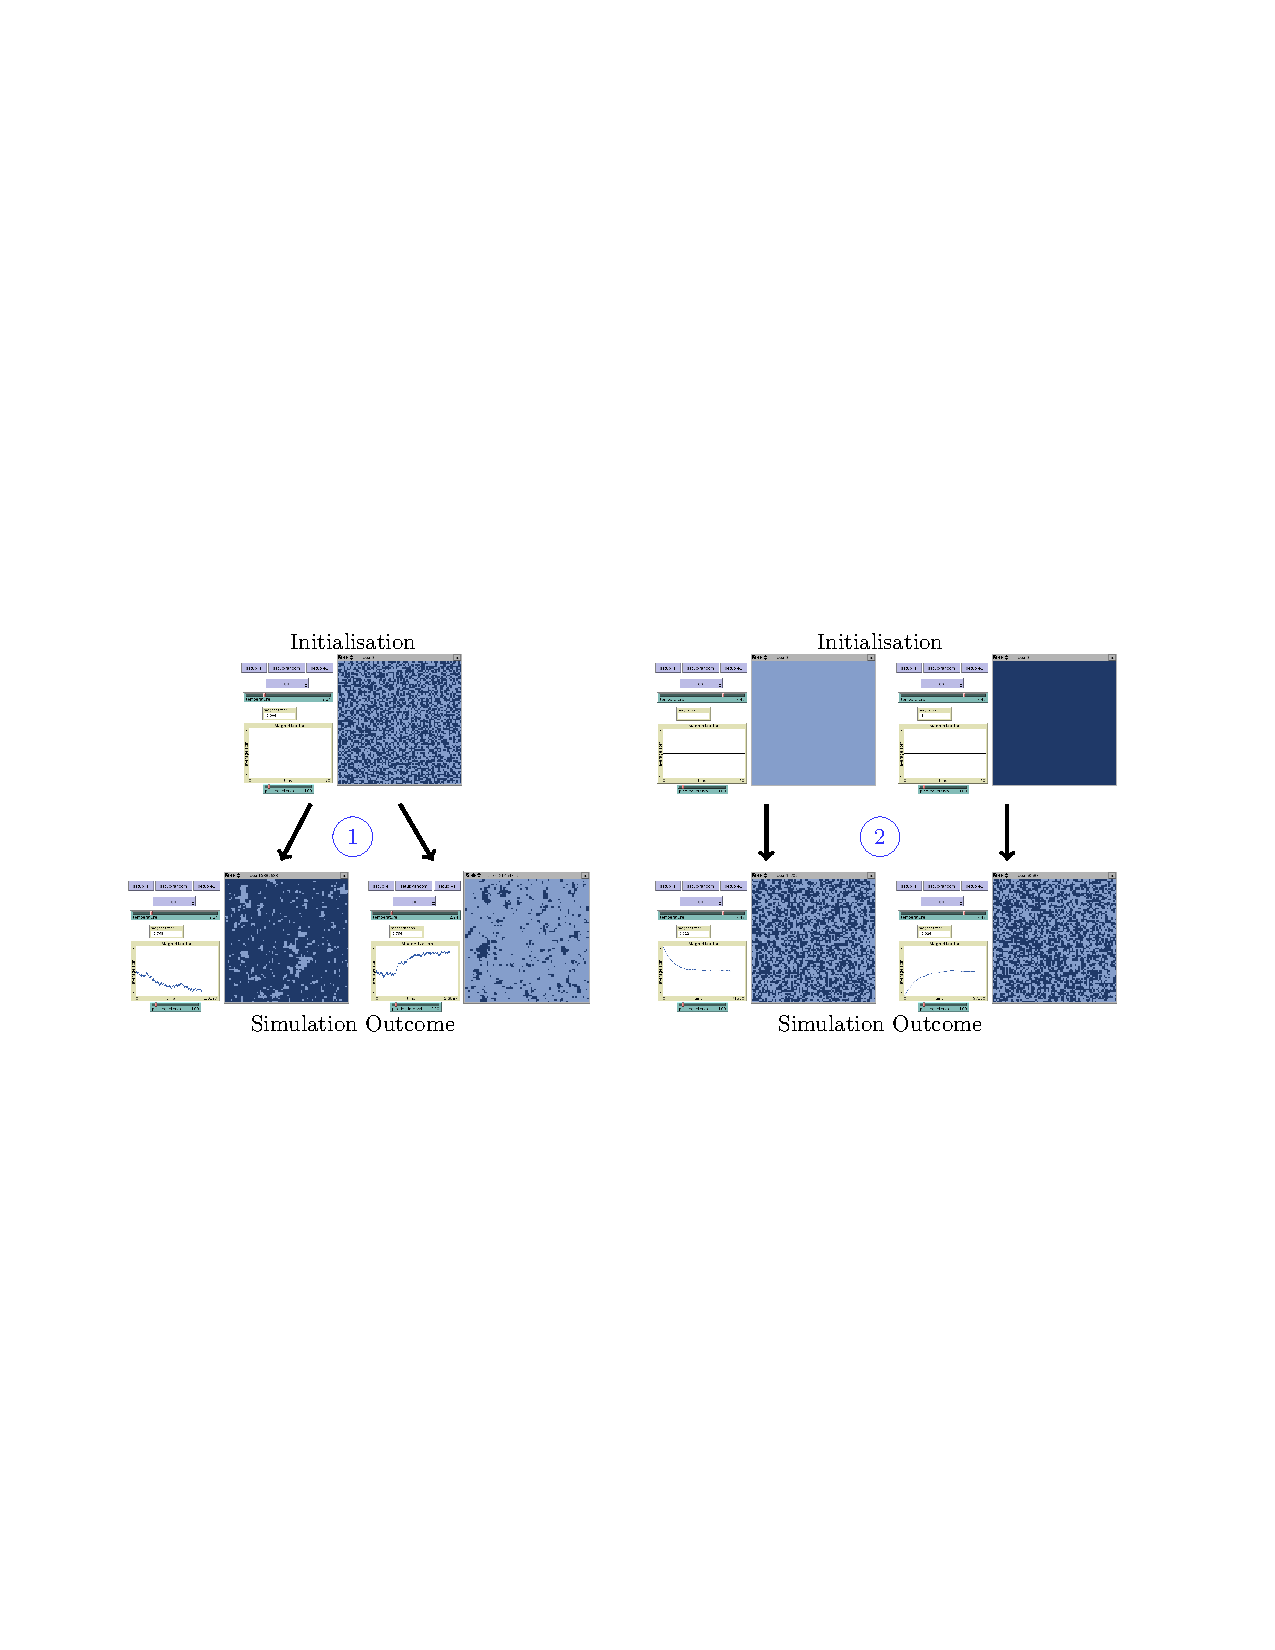
\includegraphics[width=\linewidth, trim=2cm 10cm 2cm 10cm, clip=true]{IsingSimulations}		
	\caption{Transient behaviour of the Ising model in the regions highlighted in Fig.~\ref{fig:ising}. Spontaneous magnetisation (left) and overall magnetisation of zero (right) occurring regardless of initial conditions. \label{fig:isingTransient}}
\end{figure}

As illustrated in Fig.~\ref{fig:ising}, the systems is fixed in the ferromagnetic phase ($|M|$ = $\pm 1$) where the spins of all of the atoms are aligned. Whilst in this state the magnet experiences `spontaneous magnetization' where any configuration will lead to a magnetization of $|1|$, with the sign of the $M$ depending on the initial conditions. The transient behaviour leading to convergence to one of the two solid red branches in Fig.~\ref{fig:ising} can be explained due to the presents of an unstable state at $M$=0. Here all spins are random thus there is no alignment of the atoms. Although the probability according to Equation~(\ref{eq:ising}) is low in this phase, once an atom has flipped to the lower energy spin state it will extremely unlike to flip back resulting in a slow transition from $M=0$ to $M=|1|$. This explains the observation of transitions away from $M$=0 to one of the stable branches in this temperature region. 

The system remains in the ferromagnetic phase until the temperature is above a threshold $\widetilde{T}\approx1.5$, where there is initially a strong dependency of $||M||$ with temperature. This rapid change is due to the phase shift as the system progresses into the paramagnetic state where there is no spontaneous magnetization. At $T<T'\approx2.3$ the magnet is in the paramagnetic state where all spins are randomly aligned and the state of one atom (agent) is no longer dependent on the state of its neighbours. In this region, any initial configuration of the system will always converge to a state of randomly aligned spins resulting in a magnetization of $M=0$, with the speed of convergences increases with $T$.

The point at which the system changes from ferromagnetic to paramagnetic phase, $T'$, is a bifurcation. Here the two stable branches collide with the unstable branch forming a single stable branch at $T>T'$ and is an example of a pitchfork bifurcation. Examples of the transient behaviour of the Ising model is given in Fig~\ref{fig:isingTransient} for the two phases. The number of ticks here illustrates the slow dynamics of this model, particularly in the ferromagnetic state where convergence takes 10's of millions of time steps. This indicates the issue of analysis of ABMs with simulations alone, where a single simulation takes around 40s (running at maximum speed) for this number of ticks. Then when considering repeat simulations for averaging, and parameter variation, this can rapidly become a long computational process. Equation-free methods avoid extensive computation times through short simulations from appropriate initialised settings. 
 
 
 
\section{Further Reading}

The following table contains a reference list for further reading on the topic contained in this method and example. 
\begin{center}
\begin{tabular}{|l|c|}
\hline
Topic									&	Reference \\ \hline
Introduction to bifurcation analysis		&	\cite{Meunier1988}	\\
Introduction to continuation 			&	\cite{Doedel1991,Allgower1990,Rheinboldt2000,Krauskopf2007} \\ 
Introduction to equation-free methods	&	\cite{Theodoropoulos2000,Kevrekidis2003,Kevrekidis2009}	\\
\hline
\end{tabular}
\end{center}



\section*{Acknowledgments}
{The support of the UK Engineering and Physical Sciences Research Council for programme grant EP/H021779/1 (Evolution and Resilience of Industrial Ecosystems (ERIE)) is gratefully acknowledged.}
 
 
\begin{thebibliography}{10}  

\bibitem{Netlogo}
{\sc U. Wilensky}, 
{\it NetLogo},
Center for Connected Learning and Computer-Based Modeling, Northwestern University, Evanston, IL,
http://ccl.northwestern.edu/netlogo/,
1999

\bibitem{Ising}
{\sc U. Wilensky}, 
{\it NetLogo Ising model},
Center for Connected Learning and Computer-Based Modeling, Northwestern University, Evanston, IL,
http://ccl.northwestern.edu/netlogo/models/Ising,
2003

\bibitem{Barkley2006}
{\sc D. Barkely, I. G. Keverekidis and A. M. Stuart},
{\it The Moment Map: Nonlinear Dynamics of Density Evolution via a Few Moments},
SIAM J. Applied Dynamical Systems, 2006, 5(3), pp 403-434

\bibitem{Avitabile2014}
{\sc D. Avitabile, R. Hoyle, G. Samaey},
{\it Noise reduction in coarse bifurcation analysis of stochastic agent-based models: an example of consumer lock-in},
SIAM Journal on Applied Dynamical System, 2014, ISSN 1536-0040 (In Press)

\bibitem{Meunier1988}
{\sc C. Meunier and A. D. Verga},
{\it Noise and Bifurcations}
J. Stat. Phys., 1988, 50(1-2), pp 345-375

\bibitem{Doedel1991}
{\sc E. Doedel, H. B. Keller and J. P. Kernevez},
{\it Numerical Analysis And Control of Bifurcation Problems (I) Bifurcation in Finite Dimensions}
Int. J. Bifurcation Chaos, 1991, 493(3), pp 493-520

\bibitem{Allgower1990}
{\sc E. L. Allgower and K. Georg},
{\it Numerical Continuation Methods, An Introduction}
Springer-Verlag Berlin Heidelberg 1990

\bibitem{Rheinboldt2000}
{\sc W. C. Rheinboldt},
{\it Numerical continuation methods: a perspective}
Journal of Computational and Applied Mathematics, 200, 124, pp 229-244

\bibitem{Krauskopf2007}
{\sc B. Krauskopf, H. M. Osinga and J. Gal\`{a}n-Vioque (Eds.)},
{\it Numerical Continuation Methods for Dynamical Systems}
Springer 2007

\bibitem{Theodoropoulos2000}
{\sc C. Theodoropoulos, Y. H. Qian and I. G. Kevrekidis IG}
{\it Coarse stability and bifurcation analysis using time-steppers: a reaction-diffusion example}
Proc. Natl. Acad. Sci. 2000, 97, pp 9840-9845

\bibitem{Kevrekidis2003}
{\sc I. G. Kevrekidis et al.} 
{\it Equation-free, coarse-grained multiscale computation: enabling microscopic simulators to perform system-level tasks}
Comm. Math. Sci. 2003, 1, pp 715-762 

\bibitem{Kevrekidis2009}
{\sc I. G. Kevrekidis and G. Samaey},
{\it Equation-Free Multiscale Computation: Algorithms and Applications},
Annual Review of Physical Chemistry, 2009, 60(1), pp 321-344




\end{thebibliography} 

\end{document} 

